\documentclass[a4paper,12pt]{report}
\renewcommand{\thesection}{\arabic{section}}
\renewcommand{\contentsname}{Indholdsfortegnelse}

\usepackage{apacite}
\usepackage{graphicx}
\usepackage{booktabs}
\usepackage[table,xcdraw]{xcolor}
\usepackage{float}
\restylefloat{table}

\title{T6-4 Semesterprojektrapport\\ \large Syddansk Universitet, Teknisk Fakultet,\\ Softwareteknologi og Software Engineering}
\author{
	Abdirahman Mohamed, Abdullahi\\
	\texttt{aabdi07@student.sdu.dk}
	\and
	Andersen, Mikkel Plagborg\\
	\texttt{mikke20@student.sdu.dk}
	\and
	Irvold, Anton Valdemar Dahlin\\
	\texttt{anirv20@student.sdu.dk}
	\and
	Bouzan, Jakub\\
	\texttt{jabou19@student.sdu.dk}
	\and
	Tønnes, Frederik Primdahl\\
	\texttt{frtoe20@student.sdu.dk}	 
}

\begin{document}

\date{\today}
\maketitle
\tableofcontents

\section{Introduktion}
Projektet tager udgangspunkt i de 17. verdensmål opstillet og vedtaget af alle FNs medlemslande. Verdensmålene har til formål at skabe en kurs mod en bæredygtig udvikling. Produktudformningen skal ske som et spil baseret på World of Zool frameworket.\\ 

I 2011 bestod energimixet af mere end 20\% vedvarende energi. FN’s 7. verdensmål arbejder for at skabe mere bæredygtig, pålidelig og moderne energi til et voksende energibehov.\\

Specifikt arbejder projektet med verdensmål 7.2, som fokuserer på at den fremtidige energi skal være vedvarende: “\textit{7.2 Inden 2030 skal andelen af vedvarende energi i det globale energimix øges væsentligt.}”\cite{verdensmaalene}

\section{Problemanalyse}
\subsection{Igangsættende problem}
Implementeringen af vedvarende energikilder går for langsomt.

\subsection{Identifikation}
Som identifikation af problemet, laves et problemtræ af det igangsættende problem.

\begin{figure}[H]
	\includegraphics[width=\linewidth]{images/problemtræ.jpg}
	\caption{Problemtræ over det igangsættende problem (blå). Årsager nederst (gul) og 		konsekvenser øverst (rød)}
	\label{fig:problemtræ}
\end{figure}

\subsection{Egentlige problem}
Udvikling af et læringsspil, der har til formål at informere børn og teenagere i den vestlige verden, sådan så de i fremtiden træffer de klimavenlige beslutninger, vedrørende de tilgængelige energiforsyningsmuligheder.

\subsection{Verifikation}
Problemet er givet af FN. Det antages derfor, at FN er en pålidelig institution, som har verificeret problemet i dets fulde form.

\section{Problemformulering}
\subsection{Hovedspørgsmål}
Hvordan kan man forbedre viden, om de handlemuligheder det enkelte menneske har for at påvirke udviklingen af verdensmål 7 om bæredygtig energi, gennem udvikling af et læringsspil?

\subsection{Underspørgsmål}
\begin{enumerate}
	\item Hvad handler FN’s 7. verdensmål om?
	\item Hvad er et læringsspil?
	\item Hvilke bæredygtige energikilder lever op til FN’s verdensmål?
	\item Hvordan udvikles et læringsspil, der informerer målgruppen om løsningsmulighederne?
\end{enumerate}

\subsection{Afgrænsning}
\begin{enumerate}
	\item “Følgevirkninger” er løst defineret. Projektet handler som udgangspunkt kun om de klimamæssige konsekvenser, og ikke de miljømæssige.
	\item Projektet er baseret på World of zuul-frameworket. Læringsspillet er derfor et computerspil udviklet i Java.
	\item Spillet gamificeres og dermed vil data ikke nødvendigvis følge virkeligheden fuldstændig.
	\item Projektet henvender sig til børn og teenagere, og har derfor til formål at påvirke klimaet på sigt.
	\item Projektet er baseret på de nuværende og mest udbredte energikilder.
\end{enumerate}

\section{Metode}
\subsection{Analysefasen}
I analysefasen laves der en program- og kravspecifikation, på baggrund af den indsamlede viden om problemdomænet og relevant faglig litteratur. \\
\textbf{Metoder}: Program- og kravspecifikation, verb/noun-metode \\
\textbf{Teknikker}: Hurtigskrivning, gruppeskrivning og peer review \\
\textbf{Værktøjer}: Google Docs

\subsection{Designfasen}
\textbf{Metoder}: CRC-kort, klassediagram (UML) \\
\textbf{Teknikker}: Brainstorm, filtrering, gruppeskrivning \\
\textbf{Værktøjer}: Draw.io (skitsering af diagrammer), Google Docs

\subsection{Implementeringsfasen}
\textbf{Metoder}: Objektorienteret programmering \\
\textbf{Teknikker}: Lagdeling af klasser \\
\textbf{Værktøjer}: Git, Github, GitKraken, IntelliJ, Google Docs

\subsection{Testfasen}
\textbf{Metoder}: Acceptancetest \\
\textbf{Teknikker}: Rubrics, peer review \\
\textbf{Værktøjer}: Google Docs

\section{Tidsplan}
\begin{table}[H]
\begin{tabular}{| l | l | p{7cm} |}
\hline
\textbf{Uge} & \textbf{Navn}                 & \textbf{Beskrivelse}                               \\ \hline
43           & Start på implementeringsfasen & Vejledning i klasserne. Start på 1. iteration      \\ \hline
- & Det faglige vidensgrundlag & Arbejde med projektdomænet. Indsamling af relevant faglig litteratur. \\ \hline
- & Design af løsning          & Design af løsningen ved brug af objektorienteret programudvikling     \\ \hline
44           & Dataindsamling                & Indsamling af relevant data til projektet.         \\ \hline
-            & Design af løsning             & -                                                  \\ \hline
-            & Implementering af løsning     & Løsningen udvikles i Java på baggrund af designet. \\ \hline
45           & Implementering af løsning     & -                                                  \\ \hline
46           & Implementering af løsning     & -                                                  \\ \hline
47           & Implementering af løsning     & -                                                  \\ \hline
48           & Test af løsning               & Løsningen testes ift. de opstillede krav.          \\ \hline
49           & \textit{Buffer}               & Ekstra tid til mangler.                            \\ \hline
\end{tabular}
\end{table}

\section{Faglige vidensgrundlag}
\subsection{Teori og faglig viden}
\subsubsection{Iteration 1}
For at spillet er relativt virkelighedsnært, er det nødvendigt at inddrage relevant teori og data om de valgte energikilder. Følgende information om en gennemsnitlig enhed af energikilden, er som udgangspunkt nødvendigt at kigge på: Typisk effekt/enhed, pris/effekt, CO2-forurening/energi, beskrivelse. Derudover kan følgende information også blive relevant: Konstruktionsforurening, konstruktionstid, energistabilitet/risiko, driftsomkostninger.

%indsæt tabel

Den typiske effekt pr. enhed er den typiske størrelse for kraftværket. Derfor kan kapitalprisen pr. enhed findes ved:


\subsubsection{Iteration 2}

\section{Hovedtekst}
\subsection{Analysefase}
Analysefasen af programudviklingen bruges til at få et overblik over, hvad spillet skal indeholde, og hvordan vi skal tilgå designfasen. Først brainstormede vi hvad spillet skulle gå ud på, og hvilke elementer vi gerne ville have med. Derefter blev en programspecifikation udarbejdet, som beskriver spillets handling, og de muligheder man skal have. For at begrænse spillet, og holde os inden for en realistisk tidsramme, er programspecifikationen blevet inddelt i  en “need to have”, som indeholder det nødvendige for spillets funktionalitet,  og en “nice to have”, som kan udvide spillet.\\
Derefter er der lavet en kravsspecifikation, som både indeholder de krav der er givet til projektet af SDU, og de yderligere krav, som programspecifikationen har givet. \\
Programspecifikationen er analyseret med verb/noun-metoden, hvor verber og substantiver markeres, da de kan bruges som kandidater til, hvilke metoder og klasser programmet skal indeholde.
\subsubsection{Programspecifikation}
\textbf{"Need to have"}:\\ Som spiller skal man agere som borgmester af en by. Borgmesteren har til opgave at kontrollere byens energiforsyning, sådan at byens energibehov opfyldes og byens CO2 udledning ikke bliver for høj. Borgmesteren skal derfor vælge stabile, økonomiske og klimavenlige løsninger for at vinde. Til at starte med er byens energiforsyning udelukkende sort energi. Energibehovet stiger løbende, og hvis man ikke producerer nok energi mister man penge. Man kan også tjene penge ved at producere mere energi end man har behov for. Man tjener løbende penge ved skatteindtægter. Når energibehovet når et vist punkt stopper spillet. Hvis man har holdt CO2 udledningen nede har man vundet.

\textbf{"Nice to have"}:\\ Der er begivenheder, som spilleren ikke kan forudse, som fx demonstrationer, nedsmeltninger, variation i vind og energilagring. Der er desuden flere energikilder som fx solpaneler, hydroenergi, geotermi, biomasse, naturgas, fussion, olie og naturgas. Man skal ikke kun konvertere energiforsyningen men også transportsektoren. Opgraderinger og nye energikilder kræver også at man investerer i forskning. Spillet omhandler ikke kun produktionen af strøm, men også leveringen af strømmen gennem forsyningsnettet. Dette skal holdes vedlige og udvides, så hele befolkningen har adgang til strøm.

\subsubsection{Kravspecifikation}
\textbf{Funktionelle krav}

\textbf{Non-funktionelle krav}

\subsubsection{Verb/noun-metode}
Verb/noun-metoden bruges til at finde kandidater til klasser (navneord) og metoder (udsagnsord). Navneordene og udsagnsordene er markeret i programspecifikationen nedenunder med blå (navneord) og rød (udsagnsord). \\

Der er fundet følgende navneord og udsagnsord i programspecifikationen:\\

Herefter filtreres listen over kandidater efter følgende regler:
\begin{enumerate}
	\item Ingen kopier
	\item Ingen trivielle typer
	\item Ingen tilstandsverber
	\item Find gemte udsagnsord og navneord
\end{enumerate}

\subsection{Designfase}
\subsubsection{CRC-kort}
Der udvælges herefter en række relevante klasser fra analysefasen, og der laves CRC-kort.\\

\subsubsection{Klassediagram}
\begin{figure}[H]
	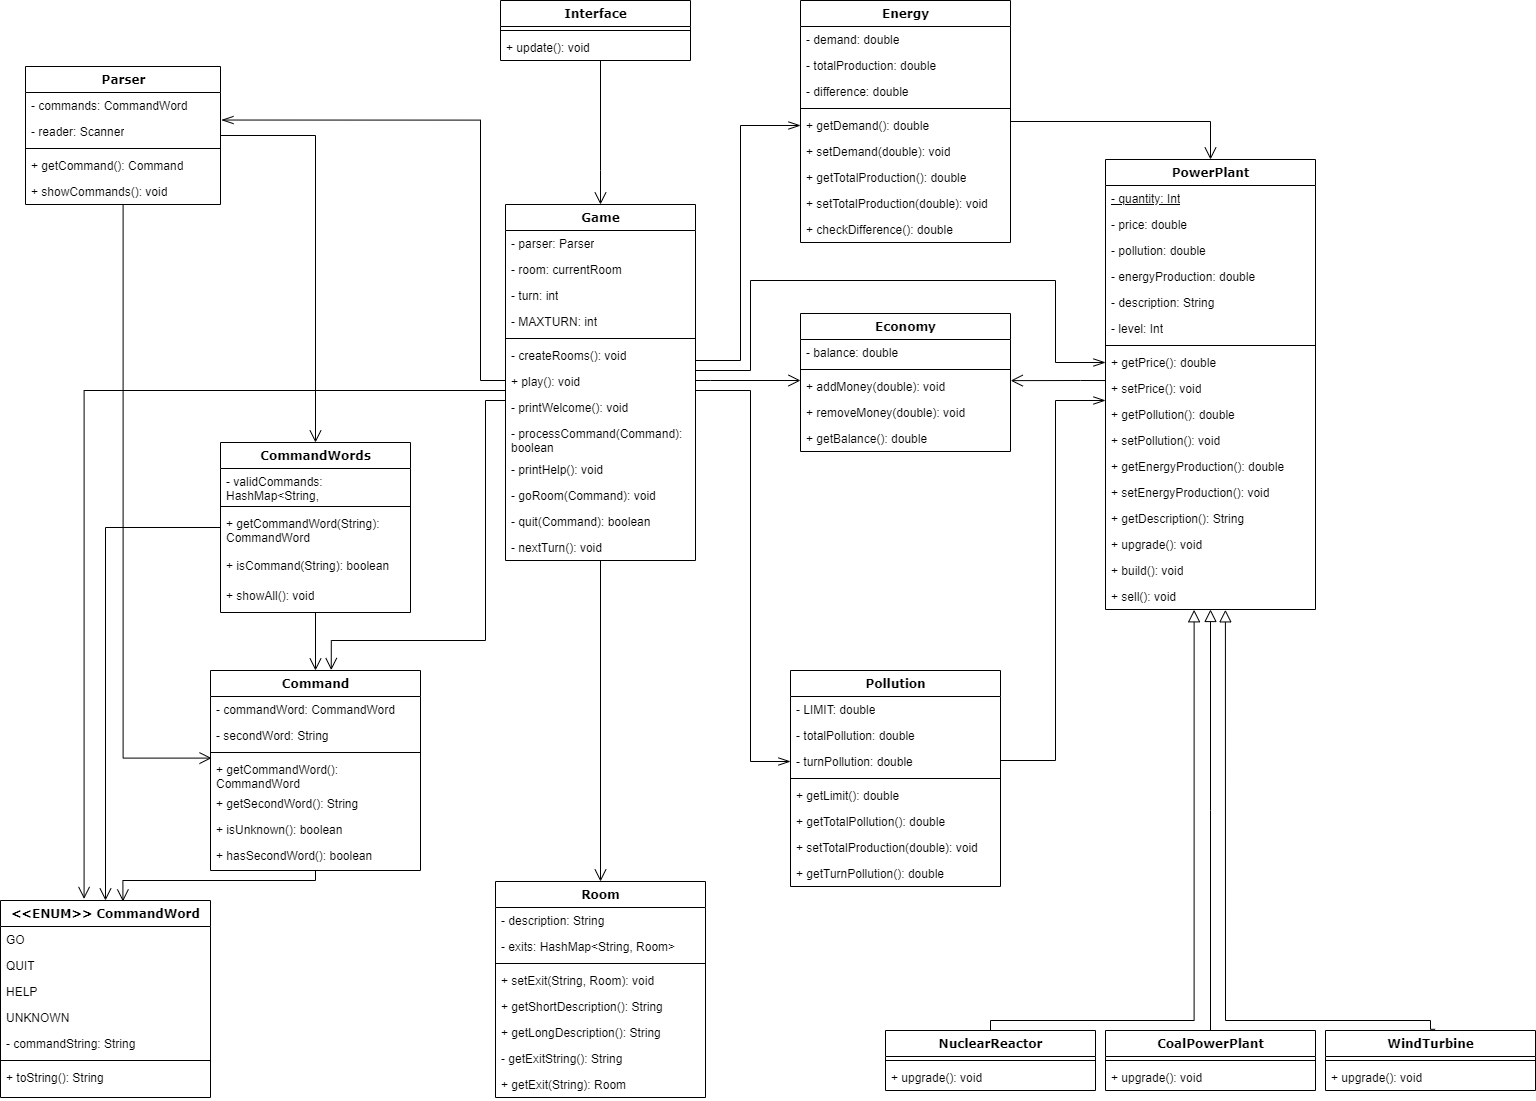
\includegraphics[width=\linewidth]{images/uml_1.png}
	\caption{Der laves et klassediagram, ud fra de overvejelser gruppen har gjort i designfasen.}
	\label{fig:uml}
\end{figure}

\bibliographystyle{apacite}
\bibliography{references}
\end{document}